\section{Rb Magneto Optical Trap}

Our journey starts with a cloud of ultracold atoms, because the tweezers are not deep enough to load room temperature atoms. Also, we need ultracold temperatures to avoid decoherence. The gas cloud is prepared using a 3D magneto optical trap (MOT). The MOT consists of 3 circularly polarized laser slightly detuned from the 780 nm D2 line of Rb-87, as well as a repump laser. The magnetic field gradient is provided by a set of coils in the standard anti-Helmholtz configuration. 

\subsection{Atom Source}

For our atom source we use a rubium dispenser. Atoms are released when the power supply is turned on. 

Here, a detailed overview will be given of the setup built for the optical tweezers experiment. The overview is split in three parts, each with their own section. 

\section{Glass Cell}

Light from a 780 Toptica laser diode is coupled in and out of a Thorlabs FC780 fiber. As it comes out of the fiber, it is sent through a polarizing beam splitter cube. To ensure maximum power transmission through the cube, the polarization of the light is rotated using a half wave plate. 

The fiber outcoupler yields a beam waist of 1.05 mm. The light is matched to the dimensions of the SLM using a Keplarian telescope consisting of a set of lenses with focal lengths $f_1=150$ mm and $f_2=500$ mm. This yields a beam waist of 1.05 mm $(f_2/f_1) \approx 3.5$ mm.

The SLM has dimensions $8$ by $15$ mm. Because this is larger than the beam waist, the power loss as a result of its aperture is limited. test

\section{Imaging Tweezer Arrays}

\section{Detecting Atoms}

The beamsize from the SLM is sent to a high numerical aperture (NA) infinity-corrected microscope objective. Additionally, it has a long working distance of 15.08 mm because it is aberration-corrected for use with a 3.5 mm cover glass. We chose the Mitutoyo G Plan Apo 50X. It's specifications are shown in \cref{table:MitutoyoSpecs}.      

\begin{table}[h]
    \caption{Mitutoyo specifications.}
    \label{table:MitutoyoSpecs}
    \centering
    \begin{tabular}{l | l}
        \textbf{Metric}                  & \textbf{Specification} \\ \hline
        NA                               & 0.5                    \\ \hline
        working distance                 & 15.08 mm               \\ \hline
        Equivalent focal length          & 4 mm                   \\ \hline
        Compatible cover glass thickness & 3.5 mm                
    \end{tabular}
\end{table}

From this we can deduct a back pupil radius $d/2 = 2 f_{\text{eff}} \text{NA} = 2$ mm. where $f_\text{{eff}}$ is the equivalent focal length. The beam from the SLM is steered to the Mitutoyo while meanwhile passing a lens relay system, mapping the SLM plane onto the back input plane of the high NA objective. 

\subsection{Relay Lenses}

The relay system serves several functions

\begin{enumerate}
    \item Avoid clipping. The SLM prints an angular phase pattern. When the distance between SLM and the objective becomes too large, the beam will clip on the pupil. The telescope is designed such that the planes at SLM and the Mitutoyo are conjugated, meaning that for any field the output is centered on the Mitutoyo. 
     
    \item Decrease beam waist. If the 3.5 mm waist from the SLM is directed to the Mitutoyo, we would lose a significant amount of power. The transmission $P/P_0 = 1- \exp{(w_i^2/R^2)} \approx 87.5\%$ for $w_i/R = 1$. Where $w_i$ is the input beam waist and $R$ the pupil radius. Therefore, the beam size is decreased by a second telescope to $w_i \approx 2$ mm.
    
    \item In an intermediate focus point in the telescope, the spot image is produced. This allows filering out unwanted diffraction orders and undiffracted light. 
\end{enumerate}

To ensure no clipping \cite{Nogrette2014}, the lenses should be placed in a 4f configuration. Additionally, the distance from the second relay to the objective should accomodate sufficient distance for the optics needed to fit in between: a polarizing beam splitter to recombine the moving beam from the acousto-optical deflectors, a dicroic mirror to split off fluoresence and a mirror to steer the beam into the vertical direction. A CAD drawing puts a conservative estimate of $f_2 \approx 400$ mm here.

Concerning the second point, the magnification $m$ should be 

\begin{equation}\label{magnification}
    m = \frac{f_2}{f_1}= \frac{R}{w(z)} \approx 0.42
\end{equation}

where $f_2$ and $f_1$ are the focal lengths of the second an first relay lenses, $R = 2$ mm is the aperture radius of the objective and $w(z) = 4.7$ mm is the beam waist from the fiber collimator. \cref{magnification} puts the total length of a full 4f relay telescope at $2f_1+2f_2 \approx 2.7$ m. 

To shorten this beam size, our partner group at University of Amsterdam make use of the versatility of the SLM to program the first relay lens in the SLM itself. However, to still satisfy all of the requirements some of the lens spacings will have to be adapted. This can be understood in terms of the ABCD matrix formalism. Consider the matrix $M$ describing a telescope with spacings according to the 4f configuration: 

\begin{equation}\label{ABCD_telescope}
    M_{4\text{f}} = 
    \begin{bmatrix}
        1 & f_2\\
        0 & 1
    \end{bmatrix}
    \begin{bmatrix}
        1 & 0\\
        -1/f_2 & 1
    \end{bmatrix}
    \begin{bmatrix}
        1 & f_1+f_2\\
        0 & 1
    \end{bmatrix}
    \begin{bmatrix}
        1 & 0 \\
        -1/f_1 & 1
    \end{bmatrix}
    \begin{bmatrix}
        1 & f_1 \\
        0 & 1
    \end{bmatrix} 
\end{equation}

Now, consider the situation where the SLM acts directly as the first lens with focal length $f_1$. Then it can be shown we have the following matrix:

\begin{equation}\label{LensSLM}
    M_{\text{SLM}} = 
    \begin{bmatrix}
        1 & L_{23}\\
        0 & 1
    \end{bmatrix}
    \begin{bmatrix}
        1 & 0\\
        -1/f_2& 1
    \end{bmatrix}
    \begin{bmatrix}
        1 & L_{12} \\
        0 & 1
    \end{bmatrix}
    \begin{bmatrix}
        1 & 0\\
        -1/f_1& 1\\
    \end{bmatrix}
\end{equation}

Solving $M_{\text{4f}} = M_{\text{SLM}}$ yields: a focal length for the second lens of $f_2 = 285$ mm, which is hard to find. However, we can enforce $f_2 = 300$ mm, relaxing requirement 1. and this will only slightly change the other parameters. Final result: $f_1 = 714$ mm, $L_{12} = 1014$ mm and $L_{23} = 426$ mm. 

\section{Rb System}

The laser system and optical frequency reference for Sr is set to arrive after this thesis was written. Additionally the atom source consisting of an oven, Zeeman slower and deflection stage was only in the design stage at the time of writing (\cref{fig:SrLoading}). Therefore, we resorted to using rubidium as an ultra cold atom source first. This allows us to test our arrays of optical tweezers. The only adjustment that needs to be done for this is the wavelength, which as it turns out happens to be minor and well within the tuning range of our titanium sapphire crystal. 

\subsection{Vacuum System and Atom Source}

The rubidium vacuum system was built by Deon Janse van Rensburg and Rik van Herk. It consists of an optically contacted glass cell (out diameter 30 mm, glass thickness 4 mm) kindly supplied by collaborators from UvA. As atom source, a triplet of Rubidium dispensers are used, powered by a power supply typically running at 5 ampères. As for pumps, a turbo pump was used for initial pumpdown to $p\sim 10^{-8}$ mbar after which an combination sputter ion pump and a non evaporative getter\footnote{NEXTorr Z 100} take over. We reached a some $p \sim 2 \cdot 10^{-10}$ mbar, after baking the system at 130${}^{\circ}$C for two weeks. This is described in the thesis of Rik van Herk \cite{Herk2022}.

\subsection{Laser System}

The atomic species that we selected to cool is \textsuperscript{85}Rb because it is the most abundant. A \textsuperscript{85}Rb requires a cooling laser detuned from the D-2 line of Rb, as well as a repump laser to cycle back atoms in the cooling transition that end up in the wrong ground state. The laser system was already in the lab, built primarily by \cite{Reijnders2010}. It used a separate repump laser (Toptica DL100, $P \sim 100$mW) from the trapping/cooling laser (Toptica DLX100, $P \sim 500$mW). 

After numerous components from the repump laser system broke, we decided to omit the seperate repump laser and put sidebands on the trapping laser using an electro optic modulator (EOM) instead, as the small amount of power lost in the trapping laser is not of critical importance for us. The laser system is sketched in \cref{fig:RbLaserSetup}. The fiber on the lower left is where previously both the trapping and repump laser would be fiber coupled for a frequency offset lock system, which we replaced by a (fiber coupled) wavemeter. 

The system consists of a laser detuned by an acousto-optic modulator. For long term stability, the laser is frequency locked using a modulation transfer spectroscopy setup \cite{McCarron2008,Reijnders2010}. In order for the laser to be in resonance with the Rb spectroscpopy cell, an AOM is used with the same frequency as the AOM going to the MOT. 

\subsection{Repump Sidebands}

In order to make the sidebands, an EOM was used. An EOM uses phase modulation to create sidebands with shifted frequencies. The amount of sidebands is determines by the modulation depth. The power in the various sidebands as a function of the modulation index $\epsilon$ is described by \cite{McCarron2008}

\begin{equation}
    E = E_0 \left[
        \sum_{n=0}^{\infty} J_n(\eta)\sin{(\omega_c+n\omega_n)t}+
        \sum_{n=1}^{\infty} (-1)^n J_n(\eta) \sin{(\omega_c-n\omega_m)t}
    \right]
\end{equation}

where $t$ is time and $\omega_c$ the carrier frequency. If $\epsilon <1$ most of the power is contained in the zeroth order (unmodulated) beam and a small fraction is contained in the first sidebands. The sidebands are always symmetric from the zeroth order, but we only use one of them, the other is wasted. 

The EOM\footnote{7Qubig EO-Rb85-3K} was fed a $f = 2915$ MHz signal provided by a harmonic synthesizer RF \footnote{DS instruments SG6000PRO} providing a signal of $-6.9$dbm. This signal was amplified by a 45 dB amplifier \footnote{Minicircuits ZHL-16W-43+} which should provide some $\sim 15$\% of power in the first sidebands \cite{Rens2014}, which should be a sufficient amount of power for a repump laser. 

\begin{figure}
    \centering
    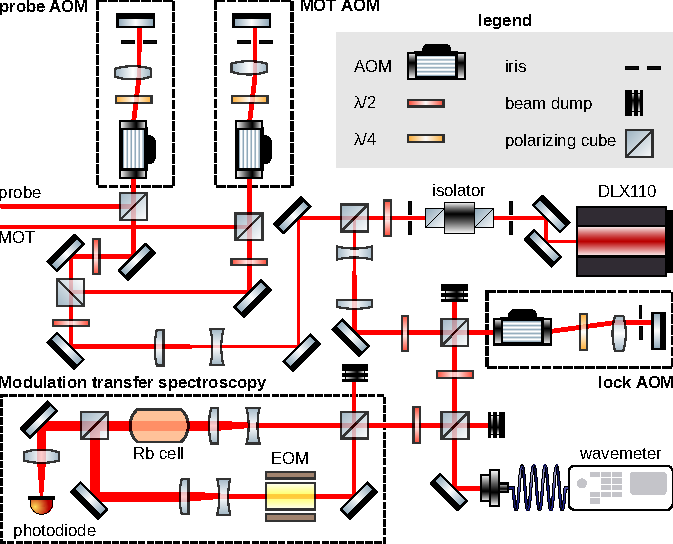
\includegraphics[width=\linewidth]{figures/RbLaserSetup.pdf}
    \caption{Laser system for the trapping and repump laser system for \textsuperscript{85}Rb. The bulk was already built by \cite{Reijnders2010}. All beam splitter cubes shown are polarizing. The Rb vapor cell is heated to 150${^{\circ}}$C.}
    \label{fig:RbLaserSetup}
\end{figure}

